\documentclass[12pt]{article}
\usepackage{geometry}
\usepackage[utf8]{inputenc}
\usepackage{a4}
\usepackage{lscape}
\usepackage{pdflscape}
\usepackage[none]{hyphenat} %hyphenation
\sloppy
\usepackage{parskip} %no indentation after paragraphs
%\usepackage{umlaute}
\usepackage{afterpage} %for using \afterpage{\clearpage} (don't push images to the end of a chapter)

%\usepackage[numbers]{natbib}  removed for \usepackage{cite}
\usepackage{graphicx}
\usepackage{picins} %provides precise control over the placement of inline graphics
\usepackage{setspace}
\usepackage{titlesec}
\usepackage{dsfont} %math symbols
\usepackage{tabularx}
\usepackage{floatflt} %float text around figures and tables
% Florian Schulze, 06.06.2012
% v1.0, latest edit: 06.06.2012

\usepackage{pdfpages}
\usepackage{enumitem} %resume counting from previous enumerate block
\usepackage{amsmath,amssymb}
\usepackage[format=default,font=footnotesize,labelfont=bf]{caption}
\usepackage{listings} %for listing source code
\usepackage{color}
\usepackage{algorithm} %wrap algpseudocode and enrich with label etc.
\usepackage{float} % for [H] after floats
\usepackage{hyperref}
\usepackage{lscape}
\usepackage{url}
\usepackage{wrapfig}
\usepackage{csquotes}
\usepackage{xfrac}
\hypersetup{
	colorlinks,
	citecolor=black,
	filecolor=black,
	linkcolor=black,
	urlcolor=black
}

\usepackage{chngcntr}
\counterwithin{table}{section}
\counterwithin{figure}{section}

\usepackage[backend=biber,
citestyle=numeric, 
bibstyle=numeric,
sorting=none,
maxbibnames=5,
urldate=comp]{biblatex}
\addbibresource{bibliography/literature.bib}

\titleformat{\section}{\vspace*{1cm}\LARGE\bfseries}{\thesection}{1em}{}
\newcommand{\sectionbreak}{\clearpage}
\titleformat*{\subsection}{\Large\bfseries}
\titleformat*{\subsubsection}{\large\bfseries}
\titleformat*{\paragraph}{\large\bfseries}
\titleformat*{\subparagraph}{\large\bfseries}


\pagestyle{plain}

\textwidth16cm
\textheight22cm


\begin{document}
	
	%\nocite{*} %include uncited references in bibliography
	\thispagestyle{empty}
	
	\pagenumbering{gobble}
	% This is tumlogo.tex
%
% Neues TUM-Logo in TeX
%   by G. Teege, 19.10.89
% Benutzung:
%   Am Anfang des Dokuments (TeX oder LaTeX):
%     \input tumlogo
%   Dann beliebig oft:
%     \TUM{<breite>}
%   bzw.
%     \oTUM{<breite>}
%   \TUM setzt das Logo mit der Breite <breite> und der entsprechenden Hoehe.
%   <breite> muss eine <dimen> sein. \oTUM erzeugt eine "outline"-Version
%   des Logos, d.h. weiss mit schwarzem Rand. Bei \TUM ist es ganz schwarz.
%   \oTUM entspricht damit der offiziellen Version des Logos.
%   Das Logo kann wie ein einzelnes Zeichen verwendet werden.
%   Beispiel:
%     Dies ist das TUM-Logo: \oTUM{1cm}.
%
\def\TUM#1{%
\dimen1=#1\dimen1=.1143\dimen1%
\dimen2=#1\dimen2=.419\dimen2%
\dimen3=#1\dimen3=.0857\dimen3%
\dimen4=\dimen1\advance\dimen4 by\dimen2%
\setbox0=\vbox{\hrule width\dimen3 height\dimen1 depth0pt\vskip\dimen2}%
\setbox1=\vbox{\hrule width\dimen1 height\dimen4 depth0pt}%
\setbox2=\vbox{\hrule width\dimen3 height\dimen1 depth0pt}%
\setbox3=\hbox{\copy0\copy1\copy0\copy1\box2\copy1\copy0\copy1\box0\box1}%
\leavevmode\vbox{\box3}}
%
\def\oTUM#1{%
\dimen1=#1\dimen1=.1143\dimen1%
\dimen2=#1\dimen2=.419\dimen2%
\dimen3=#1\dimen3=.0857\dimen3%
\dimen0=#1\dimen0=.018\dimen0%
\dimen4=\dimen1\advance\dimen4 by-\dimen0%
\setbox1=\vbox{\hrule width\dimen0 height\dimen4 depth0pt}%
\advance\dimen4 by\dimen2%
\setbox8=\vbox{\hrule width\dimen0 height\dimen4 depth0pt}%
\advance\dimen4 by-\dimen2\advance\dimen4 by-\dimen0%
\setbox4=\vbox{\hrule width\dimen4 height\dimen0 depth0pt}%
\advance\dimen4 by\dimen1\advance\dimen4 by\dimen3%
\setbox6=\vbox{\hrule width\dimen4 height\dimen0 depth0pt}%
\advance\dimen4 by\dimen3\advance\dimen4 by\dimen0%
\setbox9=\vbox{\hrule width\dimen4 height\dimen0 depth0pt}%
\advance\dimen4 by\dimen1%
\setbox7=\vbox{\hrule width\dimen4 height\dimen0 depth0pt}%
\dimen4=\dimen3%
\setbox5=\vbox{\hrule width\dimen4 height\dimen0 depth0pt}%
\advance\dimen4 by-\dimen0%
\setbox2=\vbox{\hrule width\dimen4 height\dimen0 depth0pt}%
\dimen4=\dimen2\advance\dimen4 by\dimen0%
\setbox3=\vbox{\hrule width\dimen0 height\dimen4 depth0pt}%
\setbox0=\vbox{\hbox{\box9\lower\dimen2\copy3\lower\dimen2\copy5%
\lower\dimen2\copy3\box7}\kern-\dimen2\nointerlineskip%
\hbox{\raise\dimen2\box1\raise\dimen2\box2\copy3\copy4\copy3%
\raise\dimen2\copy5\copy3\box6\copy3\raise\dimen2\copy5\copy3\copy4\copy3%
\raise\dimen2\box5\box3\box4\box8}}%
\leavevmode\box0}
% End of tumlogo.tex


\begin{center}
	\bigskip \bigskip
	\oTUM{6.0cm} \\
	\vspace*{0.8cm}
	{\huge \bf Technische Universität} \\
	\bigskip
	{\huge \bf München} \\
	\bigskip \bigskip
	{\huge \bf Department of Informatics} \\
	\bigskip
	{\Large Master Practical Course Games Engineering } \\     
	\vspace*{0.2cm}
	{\Large  Augmented Reality} \\        
	\bigskip \bigskip
	{\Large \bf Rune TD}\\
	\vspace*{0.2cm}
	{\large \bf Serious Celtic Augmented Reality Tower Defense Game} \\
	\bigskip
	\bigskip
	{\Large Summer term 2018} \\        
	\bigskip
	\begin{figure}[ht]
		\centering 
\includegraphics[width=0.15\linewidth]{figures/infologo.jpg}
	\end{figure}
	\bigskip
	{\Large \bf Authors} \\
	\vspace*{0.5cm}
	{\Large Stefan Stark, Florian Hösch}	\\
	\vspace*{0.5cm}
	{\Large Dennis-Florian Herr and Michael Felleisen}\\
	\vspace*{1cm}
	{\Large \bf Supervisors} \\
	\vspace*{0.5cm}
	{\Large Prof. Gudrun Klinker, Ph.D.}\\
	\vspace*{0.5cm}
	{\Large Dipl.-Inf. David A. Plecher, M.A.}\\
\end{center}

\vspace*{0.5cm}

	\pagenumbering{roman}
	
	\renewcommand{\thesection}{\arabic{section}}
	\newpage
	\pagenumbering{gobble}
	
	\tableofcontents
	
	\newpage
	\setlength{\baselineskip}{3ex}
	\pagenumbering{arabic}
	\setcounter{page}{2}
	\section{Introduction}
\label{sec:introduction}

\textit{``The year is 50 B.C. Gaul is entirely occupied by the Romans. Well, not entirely... One small village of indomitable Gauls still holds out against the invadors. And life is not easy for the Roman legionaries who g garrison the fortified camps of Totorum, Aquarium, Laudanum and Compendium...'', Robert Steven Caron.}~\cite{asterix-beginning}

Similar to the famous opening quote from the Asterix comics, our game is set in the middle of the last century before Christ. The Celtic culture is at its peak and shaped central Europe and the British Isles during the last centuries.~\cite{celtic-expansion} But conflict arises between the Celts and the Romans when Gaius Julius Caesar is leading his military campaigns northwards to conquer Gaul, known as the \textit{`bello Gallico'}.

During his campaigns, Caesar encounters several \textit{`oppidum'}, fortified Celtic villages or cities.~\cite{collis-oppidum} The player is taking control over the defenses of a small Celtic \textit{`oppidum'} and has to defend the village using powerful Celtic runes. After the village is fortified enough to fend of wildlife, the player has to fend of wave after wave of the Roman campaign to conquer his village. Who will come out on top? The organized roman empire or the naturalistic Celts with exceeding knowledge in ancient runes?

The game is supposed to teach players the meaning of ancient Celtic runes in a playful and engaging way. While playing the campaign players gradually unlock runes, that they must use with physical, printed markers\footnotemark \ to control the augmented reality world.
When a rune is unlocked the player gets educational information about the rune and an explanation of its effect in-game. The original meaning of the rune is related to their in-game effect to improve the learning experience by creating coherence between the educational information and the game experience.
\footnotetext{Our rune markers are explained in Chapter~\ref{sec:game_design}}

The following chapters are meant as a documentation for our prototype implementation. We start with describing the game design choices, followed by an explanation of the mechanics used to play the game. Afterwards we discuss problems during development, especially in regard to augmented reality and present a short user study of our prototype as presented at the TUM Demo Day of the summer semester 2018. Finally we discuss future work that was out of scope of the practical course.







	\section{Game Design}
\label{sec:game_design}

This chapter covers our game design in regard to game play and the educational aspect.

\subsection{General Concept}
\label{sec:game_design:subsec:general_concept}

Our game design evolves from the idea of a serious game utilizing augmented reality techniques available on larger mobile devices, i.e.\ tablets or phones with a display size of at least 7 inch.
The educational goal is to convey knowledge about Celtic runes and culture through an engaging and entertaining game experience.
Learning is supported by a connection between the matter and the game mechanic, so the player improves his skill in the game by mastering knowledge about runes and vice versa.

The game is designed as a classical Tower Defense (TD) game. Players build towers to defend their city from increasingly difficult hordes of enemies.
This is explained in more detail in Section~\ref{sec:game_design:subsec:tower_defense}.
We use augmented reality to give the player control over the towers and buildings with printed physical markers, our `rune markers' (cf. Section~\ref{sec:game_design:subsec:runes}).
This is meant to increase the learning success by bringing the runes into focus while providing a refreshing game experience through novel control mechanics.
Knowledge about runes and Celtic history is presented gradually using a game campaign, where the player unlocks new runes and additionally information after increasingly more difficult levels. This is thoroughly explained in Section~\ref{sec:game_design:subsec:campaign}.

Finally we based the style of the game on available historical data about Celtic cities, defenses and enemies, which is covered in Section~\ref{sec:game_design:subsec:history}.

\subsection{Runes and Rune Markers}
\label{sec:game_design:subsec:runes}

As the primary goal of playing the game is to learn about Celtic runes, the runes are the core of our game experience.
Therefore we split the game into two distinct phases:
A preparation phase where the player interacts with physical representations of the runes, our rune markers, and a game phase where the player interacts with the augmented reality device.

\begin{wrapfigure}{R}{0.38\textwidth}
	\centering
	
\includegraphics[width=0.35\textwidth]{figures/algiz0.jpeg}
	\caption{\label{fig:rune-marker} An Algiz rune marker for building towers}
\end{wrapfigure}

Our rune markers are printed out representations of runes that each have a unique effect in the game and need to be properly positioned by the player. Figure~\ref{fig:rune-marker} shows a rune marker for the \textit{`Algiz'} rune, which is used to build and position towers in-game.
As a player can use some runes multiple times, the rune markers have an additional unique boarder that enables the augmented reality tracking to distinguish similar runes.

As the basis for our runes and rune markers we used the 24 runes of the \textit{`Elder Futhark'}~\cite{elder-futhark}, the oldest form of the runic alphabets.
Almost\footnotemark all of the 24 runes have a special meaning in the game that closely relates to their original meaning.
For example the Algiz rune has the meanings \textit{`Elk', `Protection', `Defense'}~\cite{algiz} and is used to build towers.
Though, it must be noted here though that runes can have multiple meanings and the meaning is not always absolutely clear.
Rieckhoff and Biel point out that there is not Celtic historiography, literature or religious writings.~\cite{rieckhoff-runes} The absence of a large basis of usage, makes interpreting runes especially difficult.
\footnotetext{Unfortunately, we had to skip some runes as there was no reasonable way of mapping the rune to an in-game functionality.}
A complete table of the runes we used, the original meaning we used as a basis and their usage in-game can be found in Appendix TODO.

To properly play the game a player must recognize a rune and it's function in-game.
The player has as much time as he needs to study, recognize and properly place the runes in the preparation phase.\footnotemark
In combination with the coverage of most runes in-game and a close relation of their traditional meaning to the in-game usage, this measures support the learning success of the player.

\footnotetext{Though this can help him learn the runes, this was also a necessity due to the nature of augmented reality on a tablet computer.}

\subsection{Tower Defense}
\label{sec:game_design:subsec:tower_defense}

We use the basic and popular tower defense concepts for our core gameplay mechanics. Towers are manually placed on the map (through the position of the rune markers relative to the augmented reality map) and shoot incoming waves of enemies. The enemies have to be killed before they can reach the village, which is positioned with the \textit{`Mannaz'} rune marker and the anchor point of the augmented reality map.
If enemies reach the village, players loose health. When health reaches zero, the game is lost and the player has to start over.

Players can upgrade their towers by placing buff runes close to their tower rune. For example the \textit{`Kenaz'} rune adds fire damage to the tower it's linked to.
As enemies are vulnerable to different damage types, e.g. a wooden siege weapon is vulnerable to fire damage, players have to carefully consider their elemental upgrades.
Additionally players can earn gold by building farms and harvesting them during the game phase, which adds additional interactivity to the game phase.
The gold can be used to buy additional lives during the preparation phase.

Although, we would've liked to implement advanced mechanics we decided to stick with this basic tower defense principles, which works with our augmented reality setup and is intuitive to use, because of the difficulties encountered (cf. Section~\ref{sec:problems}).


\subsection{Campaign}
\label{sec:game_design:subsec:campaign}

The game and also the learning process is structured into increasingly difficult levels. At each level the player unlocks new runes, gets information about the runes historical meaning and it's use in-game.
E.g. in the first level the player unlocks the \textit{`Mannaz'} and \textit{`Algiz'} rune so he can build the village and his first tower. In the second level he unlocks another \textit{`Algiz'} rune for a second tower and a \textit{`Jera'} rune to build a farm he can harvest during the game phase.
The player gets textual information in a dialog window and an enlarged image of the new rune.
He has to immediately learn to recognize the rune to be able to find the rune marker with the rune and use it to construct or enhance buildings.
For additional references the player can open a \textit{`wiki'}, where he can find all information about runes and the game in a structured format.
We chose this structured campaign approach, because we quickly realized while testing that 24 runes with different meanings is overwhelming when directly available and a slower introduction in small manageable steps yields better results.

Each level also spawns new and tougher enemies, so the player is forced to use his runes wisely to beat the level and advance in the campaign.
After beating the campaign, a free-play mode is unlocked to offer a challenge with all runes available.


\subsection{Historical Reference}
\label{sec:game_design:subsec:history}

We created a mostly historical accurate setting for the game. Because we used a self-made voxel engine (cf. Section~\ref{sec:implementation:voxelframework} to render our game, we were able to create the game assets by ourselves.

Our Celtic village is based on reconstructions of the \textit{`Oppidum of Manching'} as illustrated in~\cite{kraemer-oppidum-maching}. The tower and stone walls were modeled after historically funded illustrations from~\cite{kraemer-oppidum-maching}\cite{rieckhoff-walls1}\cite{rieckhoff-walls2}\cite{rieckhoff-tower}. As enemies we created attackers that the Celts may have actually encountered.
They get attacked by wolves and bears in the beginning and later by invading Roman foot soldiers and siege weapons.
The attackers may also be accompanied by mythical creatures the Celts believed in like the Kelpie, a equine water spirit.



INSERT PICTURE HERE

INSERT SCREENSHOT HERE







	\chapter{Mechanics}

\section{Runes}

\section{Rune Combining}


	\section{Encountered Problems}

\subsection{Markertracking}

Since we were creating our project in Unity we decided to use Vuforia as our Augmented Reality tracking library, but the performance was not sufficient in the beginning.\\
The tracking was not stable enough for the amount of markers we intended to use, so we had to change a few aspects of our game.\\\\
The first thing we scraped were the enemy path markers. Instead the path spawns relative to the base rune. This solved stability issues as well as problems with very efficient path patterns made by the players.
By removing this player variable we had an easier time creating a balanced campaign mode.\\\\
The second thing we improved were the markers themselves. The first hand-drawn markers did not bring the image recognition performance we needed.\\
Therefore all the markers we used in our project were generated by a script. In the center of each marker is the central rune the marker is representing and the outlines of the marker consists of the whole rune alphabet in a random order.
Because of that, we could have multiple different instances of the same rune markers without using e.g. plain numbers.\\

\subsection{Marker printing}

The first time we printed all of the, close to 100 markers, we used a very simple printer and very basic printing paper.
This resulted in white vertical lines across most of the markers, which was very bad for the image tracking process. 
Moreover, after using the markers a few times, they started to bend which made the tracking even worse.
After that we used an industrial printer with very thick paper and got much better results in tracking and marker durability in general.

\subsection{ARCore/ARKit}

ARCore and ARKit was anounced in August 2017 and promised heavy performance boosts in the markerless tracking technology. Those advances in tracking stability could have been a great benefit for 
the game. Unfortunately, the support release for phones that are not flagship level phones (like the Galaxy S9 /iPhone 8) is still in the making. Dynamic environmental lighting and AR plane detection
were the features we especially looked forward to.


	\chapter{Userstudy}


	\section{Future Work}

\subsection{Free Play Mode}

The Free Play Mode was supposed to be played after completing the campaign. It would be designed to test and strengthen the knowledge gained about runes, their meaning and how to use them most efficiently.

To achieve this, the player would fend off randomly generated waves of enemies with all runes unlocked. Before each wave starts, information about the type of attackers is displayed in form of rune symbols and/or names. If the player was shown the runes "Ehwaz" (speed) and "Kenaz" (torch) for example, he would know to expect a wave of fast enemies with fire element and could adjust his strategies accordingly.
This mode could easily be implemented as a two player mode as well, with one player creating the waves of attackers using markers and the other fending them off.

\subsection{Wearables}

For a game like this, wearable Head Mounted Displays (HMD) could enhance the player experience quite a bit. HMDs like the Microsoft HoloLens, Oculus Rift, the HTC Vive or Google Cardboard could be used to increase immersion.
The usage of HMDs with the Unity engine is relatively easy. Player input on the other hand is a difficult task.
Using a simple mouse would break the immersion a lot. Using a controller would be acceptable, but the game requires the player to use their hands to place runes so the player would have to put down and pick up the controller constantly. Gesture recognition would be the optimal solution but is very difficult and time consuming. 

	\newpage
	\phantomsection % so hyperref can anchor to the bibliography
	\addcontentsline{toc}{section}{\bibname}
	\printbibliography 
	\clearpage
	\appendix
	\begin{center}
	\bigskip \bigskip
	{\huge \bf Appendix} \\
	\bigskip
\end{center}
\addcontentsline{toc}{section}{Appendix}

\section{Appendix A}
\label{appendix-runes}
\subsection*{Rune Table}
\begin{table}[ht]
	\centering
	{\renewcommand{\arraystretch}{1.5}
		\begin{tabular}{ | c | c | p{5.5cm} | p{7cm} | }
			\hline
			\textbf{Rune} & \textbf{Name} & \textbf{Meanings} &
			\textbf{In-game function} \\
			\hline
			\raisebox{-0.25\totalheight}{
\includegraphics[width=0.45cm]{pictures/runes/algiz.png}} &
			Algiz & \small Elk, Defencs, Protection & \small Build Tower \\
			\hline
			\raisebox{-0.25\totalheight}{
\includegraphics[width=0.45cm]{pictures/runes/berkanan.png}} &
			Berkanan & \small Birch, Birth, Earth & \small Element: Earth \\
			\hline
			\raisebox{-0.25\totalheight}{
\includegraphics[width=0.45cm]{pictures/runes/dagaz.png}} &
			Dagaz & \small Day, Light, Balance & \small Element: Light \\
			\hline
			\raisebox{-0.25\totalheight}{
\includegraphics[width=0.45cm]{pictures/runes/ehwaz.png}} &
			Ehwaz & \small Horse, Movement, Speed & \small Tower: Attackspeed \\
			\hline
			\raisebox{-0.5\totalheight}{
\includegraphics[width=0.45cm]{pictures/runes/fehu.png}} &
			Fehu & \small Cattle, Wealth, Dynamic Property & \small Farm: Cow Upgrade \\
			\hline
			\raisebox{-0.5\totalheight}{
\includegraphics[width=0.45cm]{pictures/runes/gebo.png}} &
			Gebo & \small Gift, Trade & \small Tower: Money On Hit, Village: Damage costs Money \\
			\hline
			\raisebox{-0.25\totalheight}{
\includegraphics[width=0.45cm]{pictures/runes/haglaz.png}} &
			Haglaz & \small Winter, Widespread Destruction & \small Tower: Splash Damage \\
			\hline
			\raisebox{-0.25\totalheight}{
\includegraphics[width=0.45cm]{pictures/runes/ingwaz.png}} &
			Ingwaz & \small Wine, Growth & \small Farm: Wine Upgrade \\
			\hline
			\raisebox{-0.25\totalheight}{
\includegraphics[width=0.45cm]{pictures/runes/iwaz.png}} &
			Ihwaz & \small Link & \small Tower: Enable multiple different Elements \\
			\hline
			\raisebox{-0.25\totalheight}{
\includegraphics[width=0.45cm]{pictures/runes/isaz.png}} &
			Isa & \small Ice, Freeze, Isolation & \small Tower: Slow On Hit \\
			\hline
			\raisebox{-0.25\totalheight}{
\includegraphics[width=0.45cm]{pictures/runes/jeran.png}} &
			Jera & \small Harvest, Circle of Life & \small Build Farm \\
			\hline
			\raisebox{-0.25\totalheight}{
\includegraphics[width=0.45cm]{pictures/runes/kauna.png}} &
			Kenaz & \small Fire, Torch, Ignition & \small Element: Fire \\
			\hline
			\raisebox{-0.25\totalheight}{
\includegraphics[width=0.45cm]{pictures/runes/laukaz.png}} &
			Laukaz & \small Water, River, Tears & \small Element: Water \\
			\hline
		\end{tabular}
	}
	\caption{Rune table for runes 1-14}
\end{table}


\begin{table}[H]
	\centering
	{\renewcommand{\arraystretch}{1.5}
		\begin{tabular}{ | c | c | p{5cm} | p{7cm} | }
			\hline
			\textbf{Rune} & \textbf{Name} & \textbf{Meanings} &
			\textbf{In-game function} \\
			\hline
			\raisebox{-0.5\totalheight}{
\includegraphics[width=0.45cm]{pictures/runes/mannaz.png}} &
			Mannaz & \small Human, Community, Intelligence & \small Build Village \\
			\hline
			\raisebox{-0.5\totalheight}{
\includegraphics[width=0.45cm]{pictures/runes/naudiz.png}} &
			Naudhiz & \small Distress, Hardship & \small Village: Villager defend Village, Tower: temp. SpeedUpgrade \\
			\hline
			\raisebox{-0.5\totalheight}{
\includegraphics[width=0.45cm]{pictures/runes/othalan.png}} &
			Othanal & \small Heritage, Wealth, Static Property & \small Village: inc. Money Capacity, Tower: Money on Kill \\
			\hline
			\raisebox{-0.25\totalheight}{
\includegraphics[width=0.45cm]{pictures/runes/pertho.png}} &
			Perthro & \small Luck, Destiny, Random & \small Random Upgrade Rune \\
			\hline
			\raisebox{-0.25\totalheight}{
\includegraphics[width=0.45cm]{pictures/runes/raido.png}} &
			Raido & Travel, Path & Build Path: obsolete \\
			\hline
			\raisebox{-0.5\totalheight}{
\includegraphics[width=0.45cm]{pictures/runes/sowilo.png}} &
			Sowilo & \small Sun, Warmth, targeted Power & \small Tower: Beam Upgrade, Farm: Sunflower Upgrade \\
			\hline
			\raisebox{-0.25\totalheight}{
\includegraphics[width=0.45cm]{pictures/runes/thurisaz.png}} &
			Thurisaz & \small Giant, Thorns, Defense & \small Tower: AOE around Tower\\
			\hline
			\raisebox{-0.25\totalheight}{
\includegraphics[width=0.45cm]{pictures/runes/tiwaz.png}} &
			Tiwaz & \small Sky, Honor, Discipline & \small Element: Air\\
			\hline
			\raisebox{-0.25\totalheight}{
\includegraphics[width=0.45cm]{pictures/runes/uruz.png}} &
			Uruz & \small Healing, Health  & \small Farm: Upgrade, Village: inc. max. HP\\
			\hline
			\raisebox{-0.5\totalheight}{
\includegraphics[width=0.45cm]{pictures/runes/wunjo.png}} &
			Wunjo & \small Happiness, Harmony & \small Multiple Elements, Farm: Upgrade for Sunflowerfarm \\
			
			\hline
		\end{tabular}
	}
	\caption{Rune table for runes 15-24}
\end{table}


\clearpage
\pagebreak
\section{Appendix B}
\label{appendix-illustrations}

\subsection*{Illustrations}

Illustrations as found in~\cite{kraemer-oppidum-maching}.

\begin{figure}[ht]
	\centering
	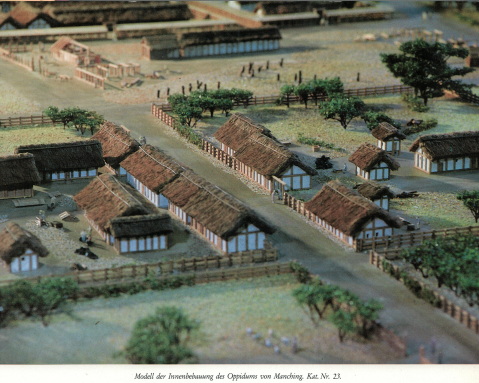
\includegraphics[width=\linewidth]{pictures/scan_manching_2.png}
	\caption{Model of the inner buildings of the  Oppodium of Manching.}
\end{figure}

\begin{figure}[ht]
	\centering
	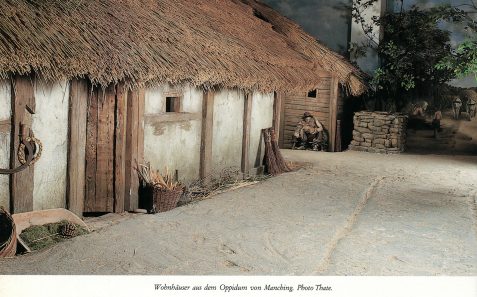
\includegraphics[width=\linewidth]{pictures/scan_manching_1.png}
	\caption{A illustration of a living house.}
\end{figure}

\begin{figure}[ht]
	\centering
	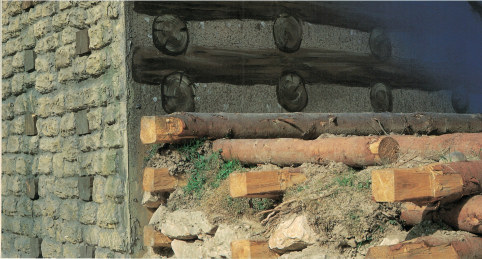
\includegraphics[width=\linewidth]{pictures/scan_manching_4.png}
	\caption{Construction of a wall.}
\end{figure}


\begin{figure}[ht]
	\centering
	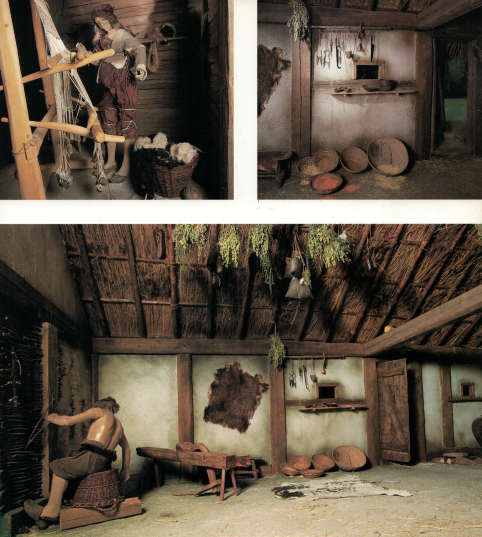
\includegraphics[width=\linewidth]{pictures/scan_manching_3.png}
	\caption{Inner view of a living house.}
\end{figure}

\clearpage
\pagebreak
Illustrations from Rieckhoff and Biel's \textit{'Die Kelten in Deutschland`}~\cite{rieckhoff-walls1}\cite{rieckhoff-walls2}\cite{rieckhoff-tower}.

\begin{figure}[ht]
	\centering
	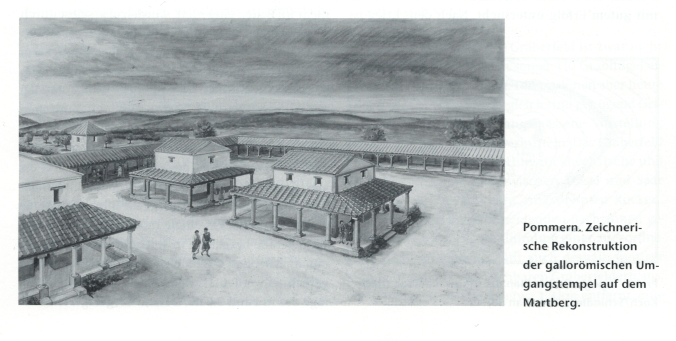
\includegraphics[width=\linewidth]{pictures/scan_rieckhoff_tower.png}
	\caption{We modeled our tower after the tower on the left of the background.}
\end{figure}

\begin{figure}[ht]
	\centering
	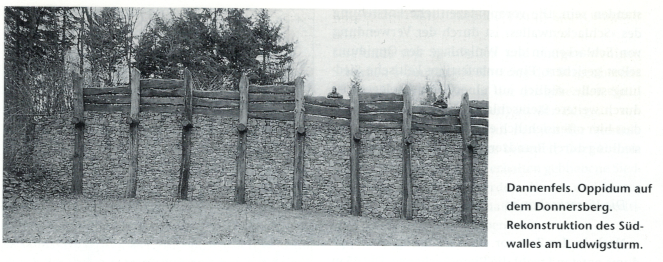
\includegraphics[width=\linewidth]{pictures/scan_rieckhoff_wall1.png}
	\caption{Reconstruction of a Oppidum wall.}
\end{figure}

\begin{figure}[ht]
	\centering
	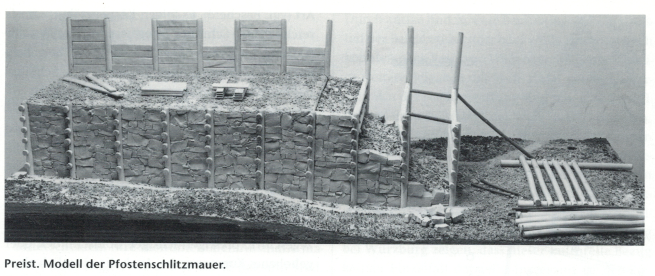
\includegraphics[width=\linewidth]{pictures/scan_rieckhoff_wall2.png}
	\caption{Another reconstruction of an Oppidum wall.}
\end{figure}

\begin{figure}[ht]
	\centering
	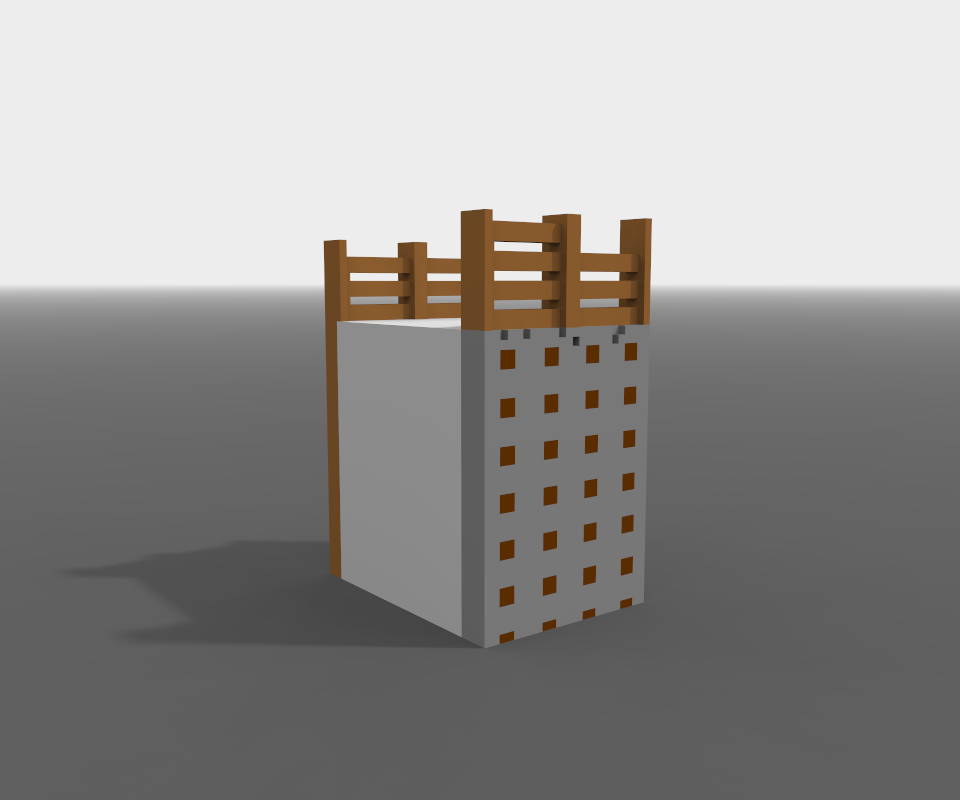
\includegraphics[width=\linewidth]{pictures/stone_wall.png}
	\caption{Our stone wall model.}
\end{figure}


\clearpage
\pagebreak
\vspace*{-3.5cm}
\section{Appendix C}
\label{appendix-userstudy}

Raw test results.

\begin{figure}[H]
	\centering
	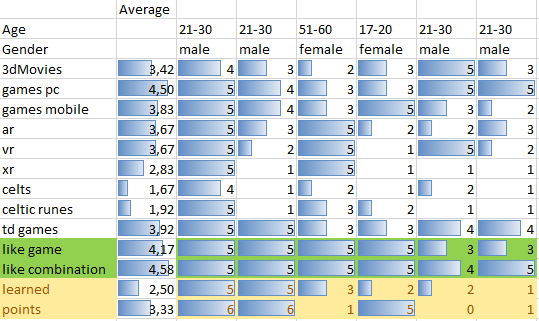
\includegraphics[width=0.95\linewidth]{figures/test-results1.png}
	\caption{Test results 1-6.}
	\label{fig:test-result1}
\end{figure}

\begin{figure}[H]
	\centering
	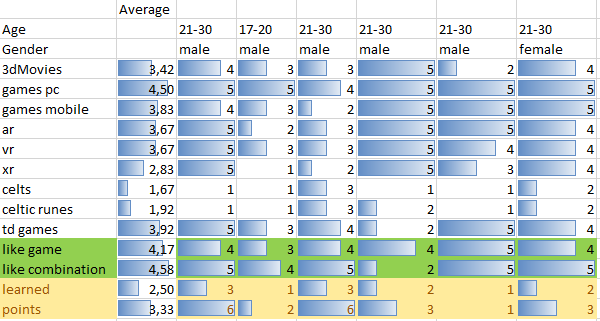
\includegraphics[width=0.95\linewidth]{figures/test-results2.png}
	\caption{Test results 7-12}
		\label{fig:test-result1}
\end{figure}



	
\end{document}

